%!TEX root = popl2018.tex

\section{Decision procedure for $\strline[\replaceall]$: The regular-expression case} \label{sec:replaceallre}

Let us consider the case that the second parameter of the $\replaceall$ function may be a regular expression.  The decision procedure presented below is a generalisation of those in Section~\ref{sec:replaceallsl} and Section~\ref{sec:replaceallcs}. 

As in previous sections, let us still start with the simple situation that $C \equiv x = \replaceall(y, e_0, z) \wedge x \in e_1 \wedge y \in e_2 \wedge z \in e_3$. For $i=0,1,2,3$, let $\cA_i = (Q_i, \delta_i, q_{0,i}, F_i)$ be the NFA corresponding to $e_i$. 

Let us first assume $\varepsilon \in \Ll(e_0)$. Then according to the semantics, for each string $u = a_1 \cdots a_n$, $\replaceall(u, e_0, v) = v a_1 v \cdots v a_n v$. Under this assumption, we can solve the satisfiability of $C$ as follows: 
\begin{enumerate}
\item Guess a set $T_z \subseteq Q_1 \times Q_1$. 
%
\item Construct $\cB_{\cA_1, \varepsilon, T_z}$ from $\cA_1$ and $T_z$ as follows: For each $(q,q') \in T_z$, add to $\cA_1$ a transition $(q, \varepsilon, q')$. Then transform the resulting NFA into one without $\varepsilon$-transitions (which can be done in polynomial time).
%
\item  Decide the nonemptiness of $\Ll(\cA_2) \cap \Ll(\cB_{\cA_1, \varepsilon, T_z})$ and $\Ll(\cA_3) \cap \bigcap \limits_{(q,q') \in T_z} \Ll(\cA_1(q,q'))$.
\end{enumerate}

Next, let us assume $\varepsilon \not \in \Ll(e_0)$. Then we know that $q_{0,0} \not \in F_0$. In addition, without loss of generality, we assume that there are no incoming transitions for $q_{0,0}$ in $\cA_0$.

To solve the satisfiability of $C$, similar to the constant-string case, we construct a parsing automaton $\cA_{e_0}$ that parses a string $v \in \Sigma^\ast e_0 \Sigma^\ast$ into $v_1 u_1 v_2 u_2 \dots v_l u_l v_{l+1}$ such that 
\begin{itemize}
	\item for each $j \in [l]$, $u_j$ is the leftmost and longest matching of $e_0$ in $(v_1 u_1 \dots v_{j-1} u_{j-1})^{-1} v$,
	%
	%\item $v_j u_j[1] \dots u_j[|u_j|-1] \not \in \Sigma^\ast e \Sigma^\ast$ for each $1 \le j \le l$, in addition, $v_{l+1} \not \in \Sigma^\ast e \Sigma^\ast$,
	\item $v_{l+1} \not \in \Sigma^\ast e_0 \Sigma^\ast$.
\end{itemize}


%
We will first give an intuitive description of the behaviour of the automaton $\cA_{e_0}$.
We will describe an automaton that can have an infinite number of states and describe the automaton as starting new ``threads''; i.e.\ run multiple copies of $\cA_0$ on the input word (similar to alternating automata).
We also describe how this automaton can be implemented using only a finite number of states.
Intuitively, in order to search for the leftmost and longest matching of $e_0$, $\cA_{e_0}$ behaves as follows.
\begin{itemize}
\item $\cA_{e_0}$ has two modes, ``$\searchleft$'' and ``$\searchlong$'', which intuitively means search for the first and last position of the leftmost and longest matching of $e_0$ respectively.
 %
	\item When in the ``$\searchleft$'' mode, $\cA_{e_0}$ starts a new thread of $\cA_0$ in each position and records \emph{the set of states} of the threads into a vector. 
    In addition, it nondeterministically makes a ``leftmost'' guessing, that is, guesses that the current position is the first position of the leftmost and longest matching. 
    If it makes such a guessing, then it enters the ``$\searchlong$'' mode, it runs the thread started in the current position and searches for the last position of the leftmost and longest matching. 
    Moreover, it stores in a set $S$ the union of the sets of states of all the threads that were started before the current position and continues running these threads to make sure that in these threads, the final states will not be reached (thus, the current position is indeed the first position of the leftmost and longest matching).
	%
	\item When in the ``$\searchlong$'' mode, $\cA_{e_0}$ runs a thread of $\cA_{0}$ to search for the last position of the leftmost and longest matching. 
    If the set of states of the thread contains a final state, then $\cA_{e_0}$ nondeterministically makes a ``longest'' guessing, that is, guesses that the current position is the last position of the leftmost and longest matching. 
    If it makes such a guessing, then it resets the set of states of the thread and starts a new round of searching for the leftmost and longest matching. 
    In addition, it stores the original set of states of the thread into a set $S$ and continues running the thread to make sure that in this thread, the final states  will not be reached (thus, the current position is indeed the last position of the leftmost and longest matching).
	%
%	\item when a thread $i$ enters a final state, a matching of $e$ is found, $\cB_e$ nondeterministically guesses whether this matching is the leftmost matching or the longest matching, 
	%
%	\item if $\cB_e$ makes a ``leftmost and longest'' guessing, then $\cB_e$ forgets all the other threads that were started later than the thread $i$, and continues running the thread $i$ and all the threads that were started earlier than the thread $i$ to make sure that final states will not be reached and the ``leftmost and longest'' guessing is correct,
%
%	\item if $\cB_e$ makes a ``leftmost and non-longest'' guessing, then $\cB_e$ forgets all the other threads that were started later than the thread $i$, and continues running all the threads that were started earlier than the thread $i$ to make sure that final states will not be reached and the ``leftmost'' guessing is correct, in addition, it continues running the thread $i$ and searching for the longest matching,
%
%	\item if $\cB_e$ makes a ``non-leftmost'' guessing, then $\cB_e$ forgets the thread $i$ and all the other threads that were started later than the thread $i$, and continues running all the threads that were started earlier than the thread $i$ and searching for the leftmost matching,
	%
	\item Since the length of the vectors of the sets of states of the threads may become unbounded, in order to obtain a finite state automaton, the following trick is applied. 
    Suppose that $S_1 S_2 \cdots S_n$ is the vector of the sets of states of the threads. 
    For each pair of indices $i, j: i < j$ and each $q \in S_i \cap S_j$, remove $q$ from $S_j$. 
    Note that the application of this trick is justified by the following arguments: Since $q$ occurs in both $S_i$ and $S_j$ and the thread $i$ was started before the thread $j$, even if from $q$  a final state can be reached in the future, the position where the thread $j$ was started \emph{cannot} be the first position of the leftmost and longest matching, since the state $q$ is also a state of the thread $i$ and the position where the thread $i$ was started is before the position where the thread $i$ was started.
\end{itemize}

In the following, we will present the construction of $\cA_{e_0}$ in detail. Before that, let us introduce some additional notation.

For $S \subseteq Q_0$ and $a \in \Sigma$, let $\delta_0(S,a)$ denote $\{q' \in Q_0 \mid \exists q \in S.\ (q,a,q') \in \delta_0 \}$. For $a \in \Sigma$ and a vector $\rho = S_1 \cdots S_n$ such that $S_i \subseteq Q_0$ for each $i \in [n]$, let $\delta_0(\rho,a)=\delta_0(S_1,a) \cdots \delta_0(S_n, a)$.

For a vector $S_1 \cdots S_n$ such that $S_i \subseteq Q_0$ for each $i \in [n]$, define $\red(S_1 \cdots S_n)$ inductively as follows:  
\begin{itemize}
\item If $n = 1$, then $\red(S_1)=S_1$ if $S_1 \neq \emptyset$, and $\red(S_1)=\varepsilon$ otherwise.
% 
\item If $n > 1$, then $\red(S_1 \cdots S_n)=\red(S_1 \cdots S_{n-1})$ if $S_n \subseteq \bigcup \limits_{i \in [n-1]} S_i$, and $\red(S_1 \cdots S_n) = \red(S_1 \cdots S_{n-1}) (S_n \setminus \bigcup \limits_{i \in [n-1]} S_i) $ otherwise.
\end{itemize}
For instance, 
%
$\red(\emptyset\{q\})=\{q\}$ and 
$$\red(\{q_1, q_2\} \{q_1, q_3\} \{q_2, q_4\})=\red(\{q_1,q_2\}\{q_1,q_3\})\{q_4\}= \red(\{q_1,q_2\}) \{q_3\} \{q_4\} = \{q_1,q_2\} \{q_3\}\{q_4\}.$$

We give the formal description of $\cA_{e_0}=(Q_{e_0}, \delta_{e_0}, q_{0,e_0}, F_{e_0})$ below.
The automaton will contain states of the form $(\rho, m, S)$ where $\rho$ is the vector $S_1\cdots S_n$ recording the set of states of the threads of $\cA_0$.
The second component $m$ is either $\searchleft$ or $\searchlong$ indicating the mode.
Finally $S$ is the set of states representing all threads for which final states must not be reached.
\begin{itemize}
	\item $Q_{e_0}$ comprises 
	\begin{itemize}
		\item the tuples $(\{q_{0,0}\}, \searchleft, S)$ such that $S \subseteq Q_0$,
		%
		\item the tuples $(\rho \{q_{0,0}\}, \searchleft, S)$ such that  $\rho = S_1 \cdots S_n$ with $n \ge 1$ satisfying that for each $i \in [n]$, $S_i \subseteq Q_0 \setminus \{q_{0,0}\}$, and for each pair of indices $i, j: i < j$, $S_i \cap S_j = \emptyset$, moreover, $S \subseteq Q_0 \setminus F_0$, 
		%
		% \item the tuples $(q_{0,e}, \longest, S)$ such that  $S \subseteq Q_e$,
		%
		\item the tuples $(S_1, \searchlong, S)$ such that $S_1 \subseteq Q_0$, $S \subseteq Q_0 \setminus F_0$ and $S_1 \not \subseteq S$;
	\end{itemize}
	%
	\item $q_{0,e_0}= (\{q_{0,0}\}, \searchleft, \emptyset)$,
	%
	\item $F_{e_0}$ comprises the states of the form $(-, \searchleft, -) \in Q_{e_0}$,
	%
	\item $\delta_{e_0}$ is defined as follows: 
	\begin{itemize}
		%\item $((q_{0,e}, \leftmost, S), a, ((\delta_e(q_{0,e},a), q_{0,e}), \leftmost, \delta_e(S,a)))$, where $\delta_e(S,a) = \{\delta_e(q,a) \mid q \in S \}$,
		%
		\item (continue $\searchleft$) suppose $(\rho \{q_{0,0}\}, \searchleft, S) \in Q_{e_0}$ such that $\rho = S_1 \cdots S_n$ with $n \ge 0$  ($n = 0$ means that $\rho$ is empty), $a \in \Sigma$, $\big(\bigcup \limits_{j \in [n]} \delta_0(S_j, a) \cup \delta_0(\{q_{0,0}\},a)\big) \cap F_0 = \emptyset$, and $\delta_0(S,a) \cap F_0 = \emptyset$, then 
		\medskip
		
		\hspace{5mm} $\left((\rho  \{q_{0,0}\}, \searchleft, S), a, \left(\red(\delta_0(\rho\{q_{0,0}\}, a)) \{q_{0,0}\}, \searchleft, \delta_0(S,a) \right) \right) \in \delta_{e_0},$
		
		\medskip
		 
		intuitively, in a state $(\rho, \searchleft, S)$, if $\big(\bigcup \limits_{j \in [n]} \delta_0(S_j, a) \cup \delta_0(\{q_{0,0}\},a)\big) \cap F_0 = \emptyset$ and $\delta_0(S,a) \cap F_0 = \emptyset$, then $\cA_{e_0}$ can choose to stay in the ``$\searchleft$'' mode,
		moreover, no states occur more than once in $\red(\delta_0(\rho \{q_{0,0}\}, a)) \{q_{0,0}\}$, since $q_{0,0}$ does not occur in $\red(\delta_0(\rho\{q_{0,0}\}, a))$, as a result of the assumption that there are no incoming transitions for $q_{0,0}$ in $\cA_0$,
        %
		\item (start $\searchlong$) suppose $(\rho \{q_{0,0}\}, \searchleft, S) \in Q_{e_0}$ such that $\rho = S_1 \cdots S_n$ with $n \ge 0$, $a \in \Sigma$, $\delta_0(S,a) \cap F_0 = \emptyset$, $\big(\bigcup \limits_{j \in [n]} \delta_0(S_j, a) \big) \cap F_0 = \emptyset$,  and $\delta_0(\{q_{0,0}\}, a) \not \subseteq \delta_0(S, a) \cup \bigcup \limits_{j \in [n]} \delta_0(S_j, a)$, then
		
		\medskip
		$\left((\rho \{q_{0,0}\}, \searchleft, S), a, \left(\delta_0(\{q_{0,0}\}, a), \searchlong, \delta_0(S, a) \cup \bigcup \limits_{j \in [n]} \delta_0(S_j, a) \right) \right) \in \delta_{e_0},$
		
		\medskip
		intuitively, from a state $(\rho \{q_{0,0}\}, \searchleft, S)$ with $\rho = S_1 \cdots S_n$, when reading a letter $a$, if $\big(\bigcup \limits_{j \in [n]} \delta_0(S_j, a) \big) \cap F_0 = \emptyset$, $\delta_0(S,a) \cap F_0 = \emptyset$, and $\delta_0(\{q_{0,0}\}, a) \not \subseteq \delta_0(S, a) \cup \bigcup \limits_{j \in [n]} \delta_0(S_j, a)$, then $\cA_{e_0}$ guesses that the current position is the first position of the leftmost and longest matching, it goes to the ``$\searchlong$'' mode, in addition, it keeps in the first component of the control state only the set of states of the thread started in the current position, and puts the union of the sets of the states of all the threads that have been started before, namely, $\bigcup \limits_{j \in [n]} \delta_0(S_j, a)$, into the third component to guarantee that none of these threads will reach a final state in the future (thus the guessing that the current position is the first position of the leftmost and longest matching is correct),


		%
		\item (continue $\searchlong$) suppose $(S_1, \searchlong, S) \in Q_{e_0}$, $\delta_0(S,a) \cap F_0 = \emptyset$, and $\delta_0(S_1,a) \not \subseteq \delta_0(S,a)$, then 
		$$((S_1, \searchlong, S), a, (\delta_0(S_1,a), \searchlong, \delta_0(S,a))) \in \delta_{e_0},$$
		intuitively, $\cA_{e_0}$ guesses that the current position is not the last position of the leftmost and longest matching and continues the ``$\searchlong$'' mode,
		%
		\item (end $\searchlong$) suppose $(S_1, \searchlong, S) \in Q_{e_0}$, $\delta_0(S_1,a) \cap F_0 \neq \emptyset$, and $\delta_0(S,a) \cap F_0 = \emptyset$, then 
		$$((S_1, \searchlong, S), a, (\{q_{0,0}\}, \searchleft, \delta_0(S,a) \cup \delta_0(S_1,a))) \in \delta_{e_0},$$
		intuitively, when $\delta_0(S_1,a) \cap F_0 \neq \emptyset$ and $\delta_0(S,a) \cap F_0 = \emptyset$, $\cA_{e_0}$ guesses that the current position is the last position of the leftmost and longest matching, resets the first component to $\{q_{0,0}\}$, goes to the ``$\searchleft$'' mode, and puts $\delta_0(S_1, a)$ to the third component to guarantee that the current thread will not reach a final state in the future (thus the guessing that the current position is the last position of the leftmost and longest matching is correct).
        %
		\item ($a$ matches $e_0$) suppose $(\rho \{q_{0,0}\}, \searchleft, S) \in Q_{e_0}$ such that $\rho = S_1 \cdots S_n$ with $n \ge 0$,  $a \in \Sigma$, $\big(\bigcup \limits_{j \in [n]} \delta_0(S_j, a) \big) \cap F_0 = \emptyset$, $\delta_0(\{q_{0,0}\}, a) \cap F_0 \neq \emptyset$, and $\delta_0(S,a) \cap F_0 = \emptyset$, then
		
		\medskip
		$\left(
		\begin{array}{l l}
		(\rho \{q_{0,0}\}, \searchleft, S), a, &\\
		& \hspace{-2cm} \left(\{q_{0,0}\}, \searchleft, \delta_0(S,a) \cup \bigcup \limits_{j \in [n]} \delta_0(S_j, a) \cup \delta_0(\{q_{0,0}\}, a) \right)
		\end{array}
		\right) \in \delta_{e_0},$
		
		\medskip
		intuitively, from a state $(\rho \{q_{0,0}\}, \searchleft, S)$ with $\rho = S_1 \cdots S_n$, when reading a letter $a$, if $\big(\bigcup \limits_{j \in [n]} \delta_0(S_j, a) \big) \cap F_0 = \emptyset$, $\delta_0(\{q_{0,0}\}, a) \cap F_0 \neq \emptyset$, and $\delta_0(S,a) \cap F_0 = \emptyset$, then $\cA_{e_0}$  guesses that $a$ is simply the leftmost and longest matching of $e_0$ (e.g. when $e_0= a$), then it directly goes to the ``$\searchleft$'' mode (without going to the ``$\searchlong$'' mode), resets the first component of the control state to $\{q_{0,0}\}$, and puts the union of the sets of the states of all the threads that have been started, including the one started in the current position, namely, $\bigcup \limits_{j \in [n]} \delta_0(S_j, a) \cup \delta_0(\{q_{0,0}\}, a)$, into the third component to  guarantee that none of these threads will reach a final state in the future (where $\bigcup \limits_{j \in [n]} \delta_0(S_j, a)$ is used to validate the leftmost guessing and $\delta_0(\{q_{0,0}\}, a)$ is used to validate the longest guessing).
	\end{itemize}
\end{itemize}

Let $Q_{\searchleft}  = \{ (-, \searchleft, -) \in Q_{e_0} \}$,  and $Q_{\searchlong} = \{ (-, \searchlong, -)  \in Q_{e_0}\}$.
Let $v = v_1 u_1 v_2 u_2 \cdots v_l u_l v_{l+1}$ such that $u_j$ is the leftmost and longest matching of $e_0$ in $(v_1 u_1 \cdots v_{j-1} u_{j-1})^{-1} v$ for each $j \in [l]$, in addition, $v_{l+1} \not \in \Sigma^\ast e \Sigma^\ast$. Then there exists a \emph{unique} accepting run $r$ of $\cA_{e_0}$ on $v$ such that the state sequence in $r$ is of the form 

\medskip
{\small
$
%\begin{array}{l}
(\{q_{0,0}\}, \searchleft, \emptyset)\ r_1\ ( \{q_{0,0}\}, \searchleft, -) \ r_2\ ( \{q_{0,0}\}, \searchleft, -)
\cdots r_l\ ( \{q_{0,0}\}, \searchleft, -)\ r_{l+1},
%\end{array}
$
}
\medskip

where for each $j \in [l]$, $r_j \in \Ll((Q_{\searchleft})^* \concat (Q_{\searchlong})^*)$, and $r_{l+1} \in \Ll((Q_{\searchleft})^*)$. Intuitively, each occurrence of the state subsequence from $\Ll((Q_{\searchlong})^* \concat (\{q_{0,0}\}, \searchleft,-))$, except the first one, witnesses the \emph{leftmost and longest} matching of $e_0$ in $v$ from the beginning or after the previous such a matching.

Since in the first component $\rho q_{0,0}$ of each state of $\cA_{e_0}$, no states from $\cA_0$ occur more than once,  it is not hard to see that $|\cA_{e_0}|$ is $2^{O(p(|\cA_0|))}$ for some polynomial $p$. 

%exponential in $|\cA_0|$. More precisely, the first components $\rho q_{0,0}$ of the control states of $\cA_{e_0}$ may take at most $\sum \limits_{i \in [|Q_0|-1]} (i+1)^{|Q_0|}$ values 

\begin{example}\label{exmp-pa-re}
Let $e_0 = 0^*0 1(1^* + 0^*)$. Then $\cA_{0}$ and $\cA_{e_0}$ are illustrated in Figure~\ref{fig-pa-re}, where ${\sf sleft}$ and ${\sf slong}$ are the abbreviations of $\searchleft$ and $\searchlong$ respectively. Let us use the state $(\{q_{0,1}\}\{q_{0,0}\}, {\sf sleft}, \emptyset)$ to illustrate the construction. Since $\big(\delta_0(\{q_{0,1}\}, 0) \cup \delta_0(\{q_{0,0}\}, 0)\big) \cap F_0 = \{q_{0,1}\} \cap F_0 = \emptyset$, $\delta_0(\emptyset, 0) \cap F_0 = \emptyset$, and $\red(\delta_0(\{q_{0,1}\}, 0) \delta_0(\{q_{0,0}\}, 0))=\{q_{0,1}\}$, we deduce that the transition $((\{q_{0,1}\}\{q_{0,0}\}, {\sf sleft}, \emptyset), 0, (\{q_{0,1}\} \{q_{0,0}\}, {\sf sleft}, \emptyset)) \in \delta_{e_0}$. On the other hand, it is impossible to go from the state $(\{q_{0,1}\}\{q_{0,0}\}, {\sf sleft}, \emptyset)$ to the ``$\searchlong$'' mode. This is due to the fact that $\delta_0(\{q_{0,0}\}, 0)=\{q_{0,1}\} \subseteq \delta_0(\{q_{0,1}\},0)=\{q_{0,1}\}$. In addition, there are no $1$-transitions out of $(\{q_{0,1}\}\{q_{0,0}\}, {\sf sleft}, \emptyset)$. This is due to the fact that $\delta_0(\{q_{0,1}\}, 1) \cap F_0 = \{q_{0,2}, q_{0,3}\} \cap F_0 \neq \emptyset$.
%
\begin{figure}[htbp]
\begin{center}
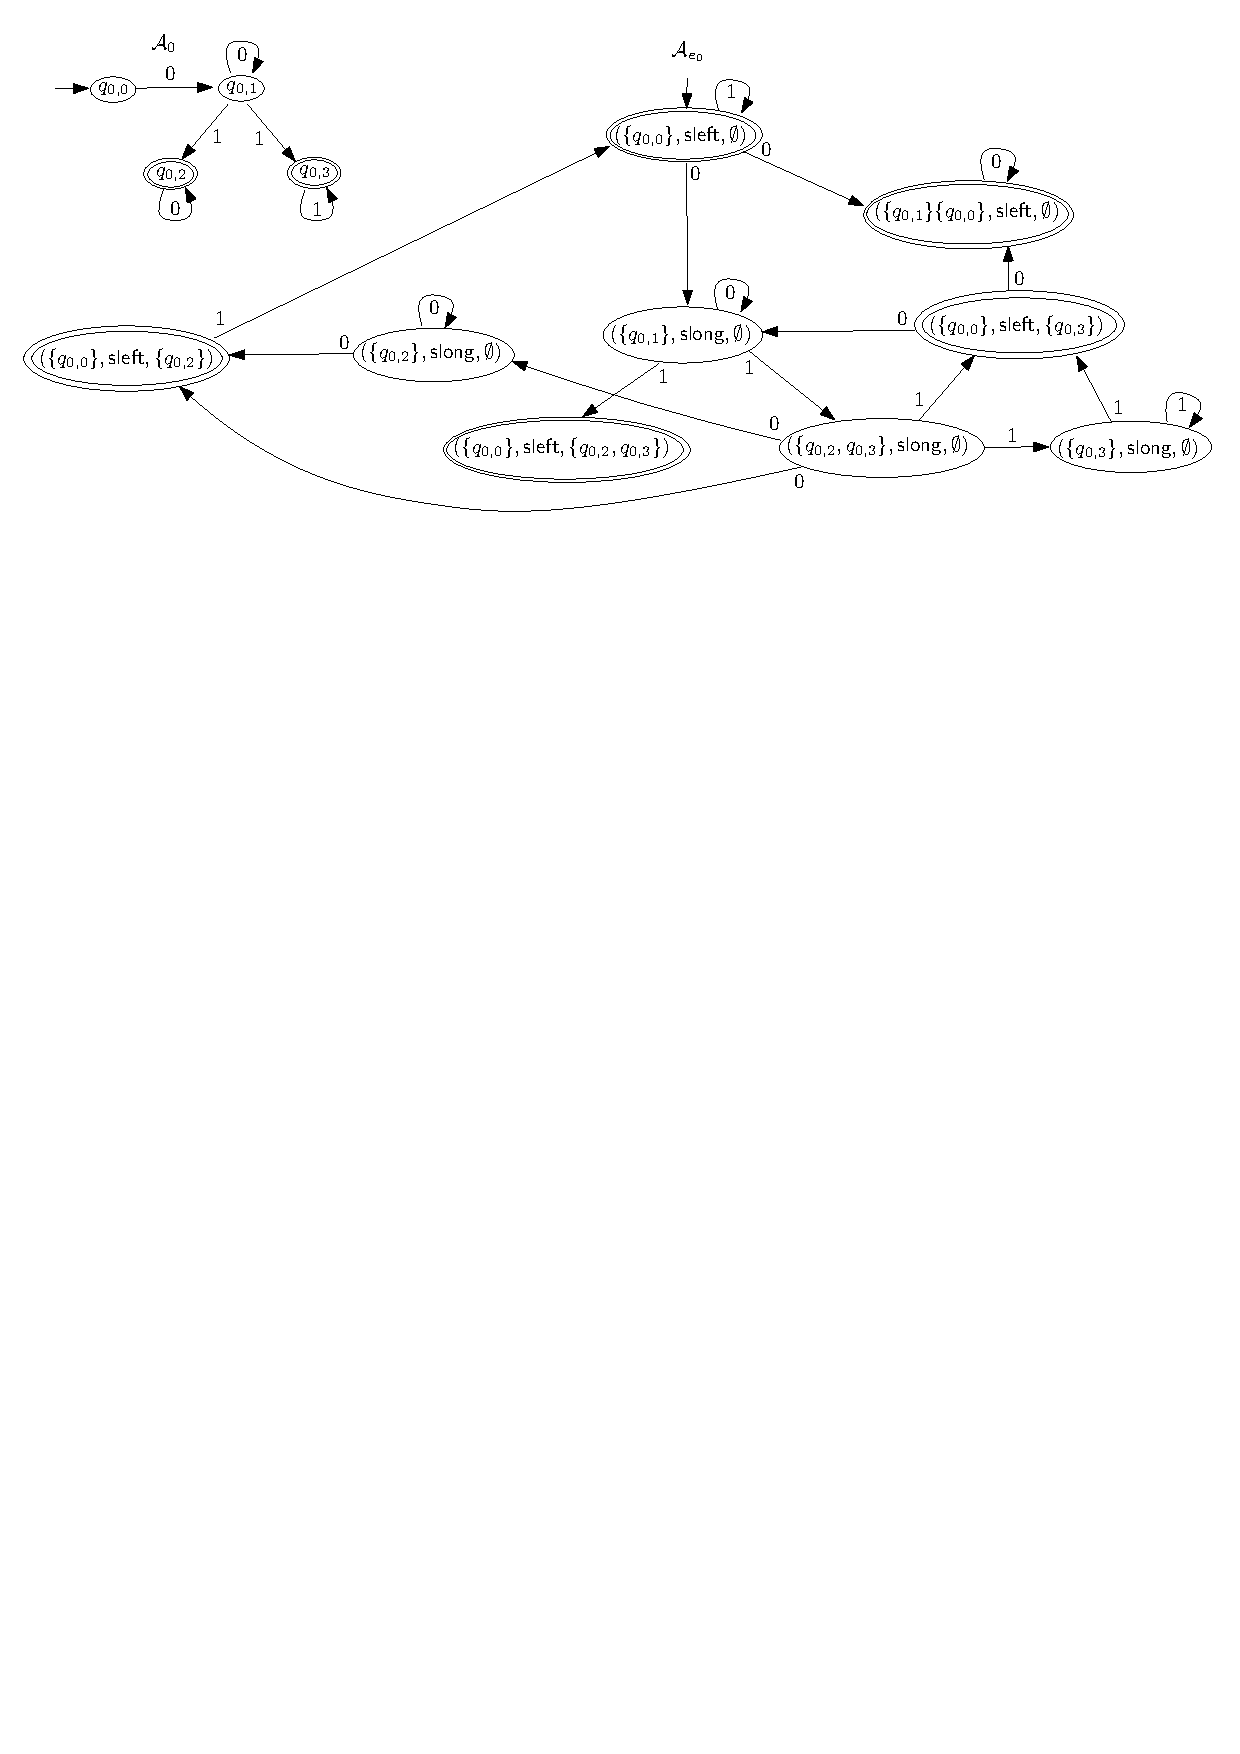
\includegraphics[scale=0.7]{regular-expression-example.pdf}
\end{center}
\caption{The NFA $\cA_0$ and $\cA_{e_0}$ for $e_0 = 0^*0 1(1^* + 0^*)$}\label{fig-pa-re}
\end{figure} 
\end{example}

Given $T_z \subseteq Q_1 \times Q_1$, we construct $\cB_{\cA_1, e_0,  T_{z}}$ by  the following three-step procedure.
\begin{enumerate}
\item Construct the product of $\cA_1$ and $\cA_{e_0}$. 

\item Remove all the transitions associated with the states from $Q_1 \times Q_{\searchlong}$, in addition, remove all the transitions of the form $((q, (\rho\{q_{0,0}\}, \searchleft, S)), a, (q', (\{q_{0,0}\}, \searchleft,S')))$ such that $\delta_0(q_{0,0},a) \cap F_0 \neq \emptyset$.

\item For each pair $(q,q') \in T_{z}$, do the following,
\begin{itemize}
\item for each transition

\medskip

$\left((\rho \{q_{0,0}\}, \searchleft, S), a, \left(\delta_0(\{q_{0,0}\}, a), \searchlong, \delta_0(S, a) \cup \bigcup \limits_{j \in [n]} \delta_0(S_j, a) \right) \right) \in \delta_{e_0}$,

\medskip

add a transition

\medskip

$\left( \left(q, (\rho \{q_{0,0}\}, \searchleft, S) \right), a, \left(q, \left(\delta_0(\{q_{0,0}\}, a), \searchlong, \delta_0(S, a) \cup \bigcup \limits_{j \in [n]} \delta_0(S_j, a) \right) \right) \right)$,

\medskip

%
\item for each transition
		$$((S_1, \searchlong, S), a, (\delta_0(S_1,a), \searchlong, \delta_0(S,a))) \in \delta_{e_0},$$
add a transition 
$$\left((q, (S_1, \searchlong, S)), a, (q, (\delta_0(S_1,a), \searchlong, \delta_0(S,a))) \right),$$
%
\item for each transition
		$$((S_1, \searchlong, S), a, (\{q_{0,0}\}, \searchleft, \delta_0(S,a) \cup \delta_0(S_1,a))) \in \delta_{e_0},$$
add a transition
		$$((q, (S_1, \searchlong, S)), a, (q', (\{q_{0,0}\}, \searchleft, \delta_0(S,a) \cup \delta_0(S_1,a)))),$$
%
\item for each transition

\medskip

		$\left(
		\begin{array}{l l}
		(\rho \{q_{0,0}\}, \searchleft, S), a, &\\
		& \hspace{-2cm} \left(\{q_{0,0}\}, \searchleft, \delta_0(S,a) \cup \bigcup \limits_{j \in [n]} \delta_0(S_j, a) \cup \delta_0(\{q_{0,0}\}, a) \right)
		\end{array}
		\right) \in \delta_{e_0},$

\medskip

add a transition

\medskip
		$\left(
		\begin{array}{l l}
		(q, (\rho \{q_{0,0}\}, \searchleft, S)), a, &\\
		& \hspace{-2cm} \left(q', \left(\{q_{0,0}\}, \searchleft, \delta_0(S,a) \cup \bigcup \limits_{j \in [n]} \delta_0(S_j, a) \cup \delta_0(\{q_{0,0}\}, a) \right)\right)
		\end{array}
		\right).$
\medskip

\end{itemize}
\end{enumerate}
Since $|\cA_{e_0}|$ is $2^{O(p(|\cA_0|))}$, it follows that $|\cB_{\cA_1, e_0, T_z}|$ is $|\cA_1| \cdot 2^{O(p(|\cA_0|))}$. In addition, since $|\cA_0|=O(|e_0|)$, we deduce that $|\cB_{\cA_1, e_0, T_z}|$ is $|\cA_1| \cdot 2^{O(p(|e_0|))}$.

\begin{example}
Let $C \equiv x = \replaceall(y, e_0, z) \wedge x \in e_1 \wedge y \in e_2 \wedge z \in e_3$, where $e_1,e_2,e_3$ are as in Example~\ref{exmp-sl} (cf. Figure~\ref{fig-sl-exmp}) and $e_0$ is as in Example~\ref{exmp-pa-re} (cf. Figure~\ref{fig-pa-re}). Suppose $T_z = \{(q_0, q_0), (q_1, q_2)\}$. Then the NFA $\cB_{\cA_1, e_0, T_z}$ is as illustrated in Figure~\ref{fig-re-exmp}, where the thick edges denote the added transitions. Let us use the state $(q_1, (\{q_{0,0}\}, \searchleft, \emptyset))$ to exemplify the construction. The transition $((q_1, (\{q_{0,0}\}, \searchleft, \emptyset)), 1, (q_2, (\{q_{0,0}\}, \searchleft, \emptyset)))$ is  in $\cA_1 \times \cA_{e_0}$. Since $\delta_0(q_{0,0}, 1) \cap F_0 = \emptyset$, this transition is not removed and is thus in $\cB_{\cA_1, e_0, T_z}$. On the other hand, since there are no $0$-transitions out of $q_1$ in $\cA_1$, there are no $0$-transitions from $(q_1, (\{q_{0,0}\}, \searchleft, \emptyset))$ to some state from $Q_{\searchleft}$ in $\cB_{\cA_1, e_0, T_z}$. 
Moreover, because $((\{q_{0,0}\}, \searchleft, \emptyset), 0, (\{q_{0,1}\}, \searchlong, \emptyset)) \in \delta_{e_0}$ and $(q_1, q_2) \in T_z$, the transition $((q_1, (\{q_{0,0}\}, \searchleft, \emptyset)), 0, (q_1, (\{q_{0,1}\}, \searchlong, \emptyset)))$ is added. 
One may also note that there are no 0-transitions from $(q_2, (\{q_{0,0}\}, \searchleft, \emptyset))$ to the state $(q_2, (\{q_{0,1}\}, \searchlong, \emptyset))$, because there are no pairs $(q2,-) \in T_z$.
It is not hard to see that $010101 \in \Ll(\cA_2) \cap \Ll(\cB_{\cA_1, e_0, T_z})$. In addition, $10 \in \Ll(\cA_3) \cap \Ll(\cA_1(q_0,q_0)) \cap \Ll(\cA_1(q_1,q_2))$. Let $y$ be $010101$ and $z$ be $10$. Then $x$ takes the value $\replaceall(010101, e_0, 10)=10 \cdot \replaceall(101, e_0, 10)=10110$, which is accepted by $\cA_1$. Therefore, $C$ is satisfiable.
\begin{figure}[htbp]
\begin{center}
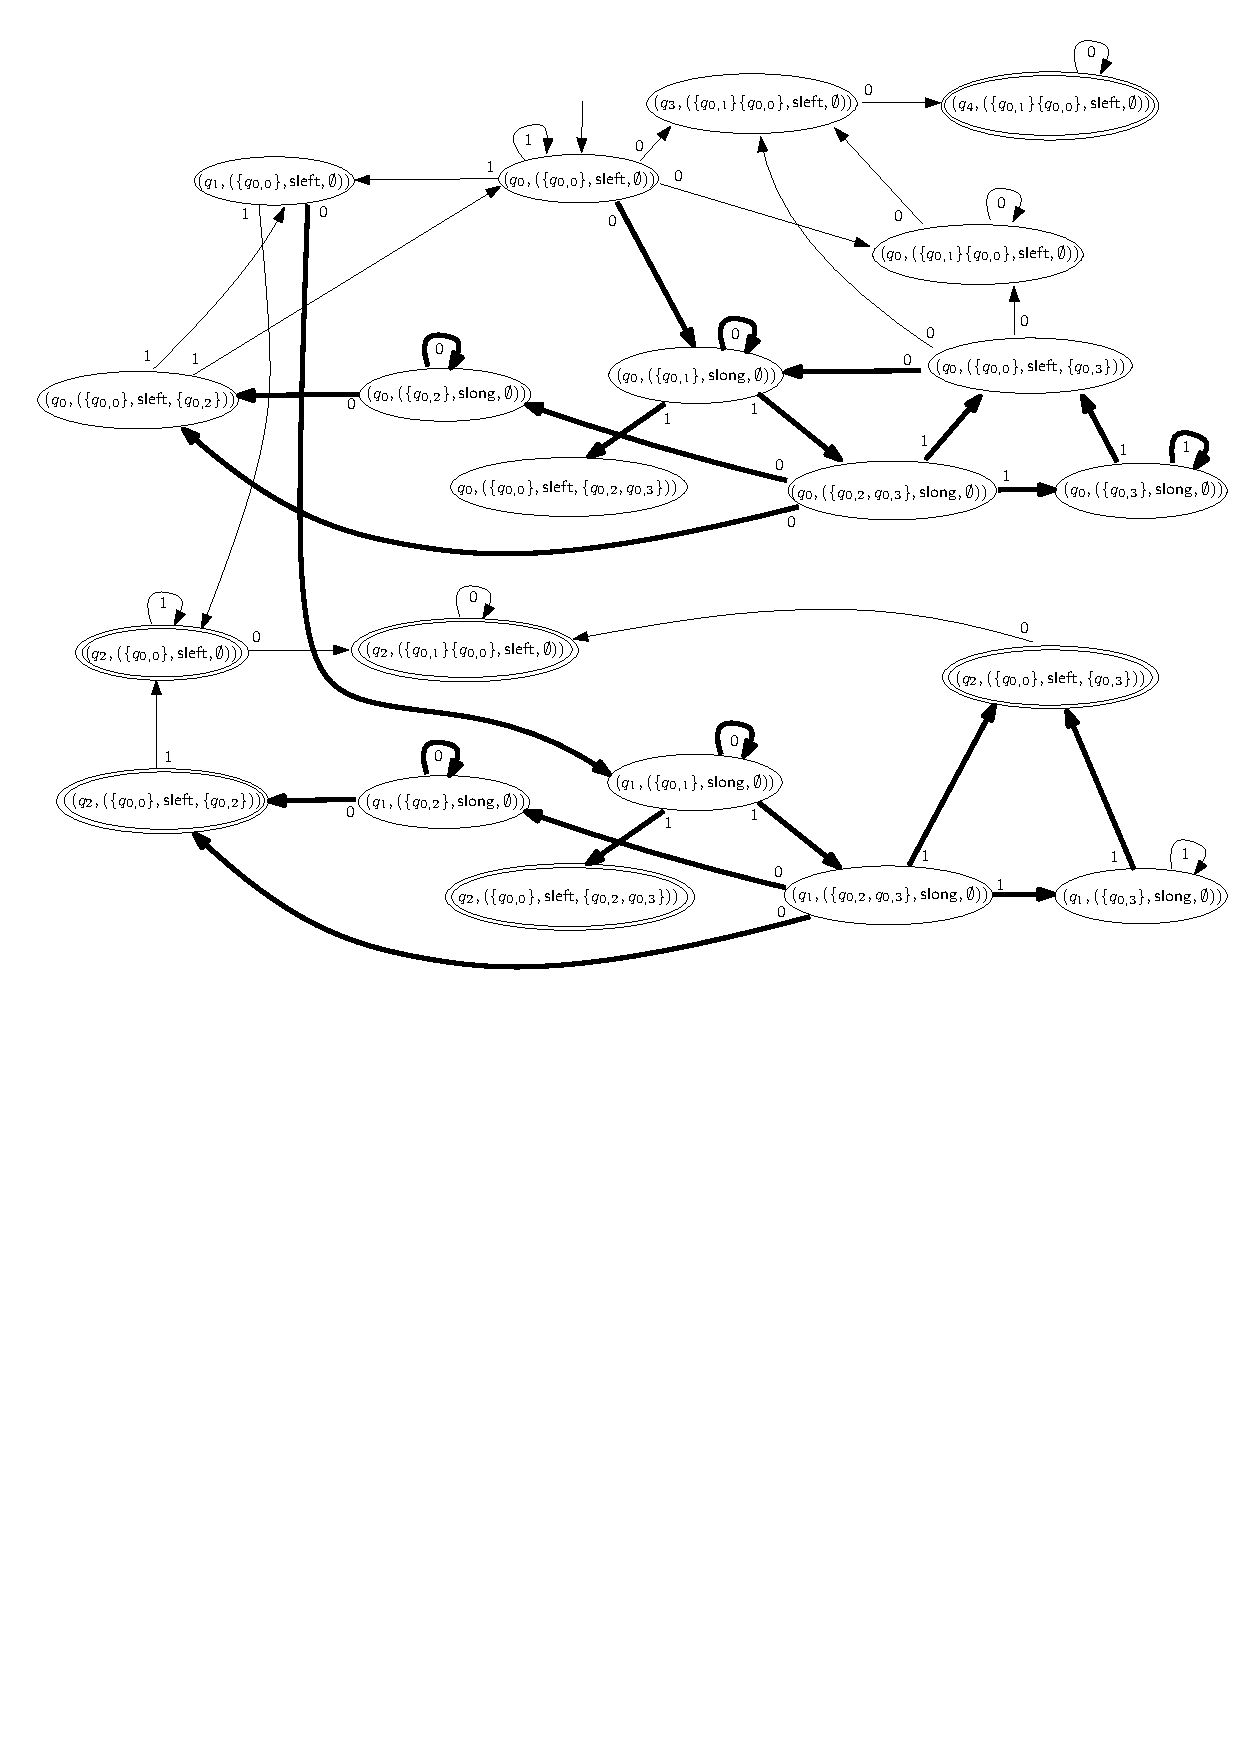
\includegraphics[scale=0.68]{regular-expression-example-2.pdf}
\end{center}
\caption{The NFA $\cB_{\cA_1, e_0, T_z}$}\label{fig-re-exmp}
\end{figure} 
\end{example}

For the more general case that the $\strline[\replaceall]$ formula $C$ contains more than one occurrence of $\replaceall(\cdots)$ terms, we still nondeterministically remove the edges in the dependency graph $G_C$ in a top-down manner and reduce the satisfiability of $C$ to the satisfiability of a collection of regular constraints for source variables. 

\paragraph*{Complexity}
In each step of the reduction, suppose the two edges out of $x$ are currently removed, let the two edges be from $x$ to $y$ and $z$ and labeled by $({\sf l}, e)$ and $({\sf r}, e)$ respectively, then each element of $(\cT, \cP)$ of $\cE_i(x)$ may be transformed into an element $(\cT',\cP')$ of $\cE_{i+1}(y)$ such that $|\cT'| = |\cT| \cdot 2^{O(p(|e|))}$, meanwhile, it may also be transformed into an element $(\cT'',\cP'')$ of $\cE_{i+1}(y)$ such that $\cT''$ has the same state space as $\cT$. Thus, after the reduction, for each source variable $x$, $\cE(x)$ may contain exponentially many elements, and each of them may have a state space of exponential size, more precisely, if we start from a vertex $x$ without predecessors, with an element $(\cT,\cP)$ in $\cE_0(x)$, and go to a source variable $y$ through a path where $k$ edges have been traversed and removed, let $e_1,\cdots, e_k$ be the regular expressions occurring in the labels of these edges, then the resulting element in $\cE(y)$ has a state space of size $|\cT| \cdot 2^{O(p(|e_1|))} \cdot 2^{O(p(|e_2|))} \cdot \cdots \cdot 2^{O(p(|e_k|))}$ in the worst case. To solve the nonemptiness problem of the intersection of all these regular constraints, the exponential space is sufficient. Consequently, for the most general case of regular expressions, we still obtain a EXPSPACE upper bound. 

On the other hand, for the situation that the $\rpleft$-length of $G_C$ is at most one, we wan to show that the algorithm runs in polynomial space. Suppose the $\rpleft$-length of $G_C$ is at most one. Then the diamond index of $G_C$ is at most one as well. According to Proposition~\ref{prop-di}, there are only polynomially many paths in $G_C$. Nevertheless, for each source variable $x$, $\cE(x)$ may contain an element $(\cT,\cP)$ such that $|\cT|$ is exponential. Since $|\cP|$ may be exponential, $(\cT,\cP)$ may correspond to the intersection of exponentially many regular constraints. However, we can show that $|\cP|$ is at most polynomial, as a result of the fact that the $\rpleft$-length of $G_C$ is at most one. The arguments proceed as follows: Suppose two edges from $x$ to $y, z$ respectively are removed, and an element $(\cT', \cP')$ of $\cE_{i+1}(y)$ such that $|\cT'|$ is exponential and $|\cP'|$ is polynomial, is generated from an element of $(\cT, \cP)$ of $\cE_i(x)$. Then $y$ must be a source variable in $G_C$. Otherwise, there is an $\rpleft$-edge out of $y$ and the $\rpleft$-length of $G_C$ is at least two, a contradiction. Therefore, $y$ is a source variable in $G_C$, $(\cT', \cP')$  will not be used to generate the regular constraints for the other variables. In other words, $y$ is a source variable in $G_C$, and $(\cT', \cP') \in \cE(y)$ with $|\cP'|$ polynomial. We then conclude that for each source variable $x$, $|\cE(x)|$  is at most polynomial in the size of $C$ and for each element $(\cT, \cP) \in \cE(x)$, $|\cP|$ is polynomial in the size of $C$. Therefore, for each source variable $x$,  $\cE(x)$ corresponds to the intersection of polynomially many regular constraints, where each of them has a state space at most exponential size. To solve the nonemptiness of the intersection of these regular constraints, the polynomial space is sufficient. We obtain a PSPACE upper bound for the situation that the $\rpleft$-length of $G_C$ is at most one.

%\subsection{A decision procedure for $\strline[\replaceall]$}


